\documentclass[12pt,one side]{article}\usepackage[utf8]{inputenc}\usepackage[a4 paper]{geometry}\usepackage{graphicx, setspace, appendix, mathrsfs, enumerate,amsmath, amsfonts, array, tabularx, longtable, rotating, caption, mathtools}\usepackage[english]{babel}\renewcommand{\baselinestretch}{1.25}\doublespacing\title{Data analysis}\author{Yao Luo}\begin{document}\maketitle
\section{Empirical distribution}
In 2023, the distribution of exam scores is:
\begin{figure}[h!]
\centering
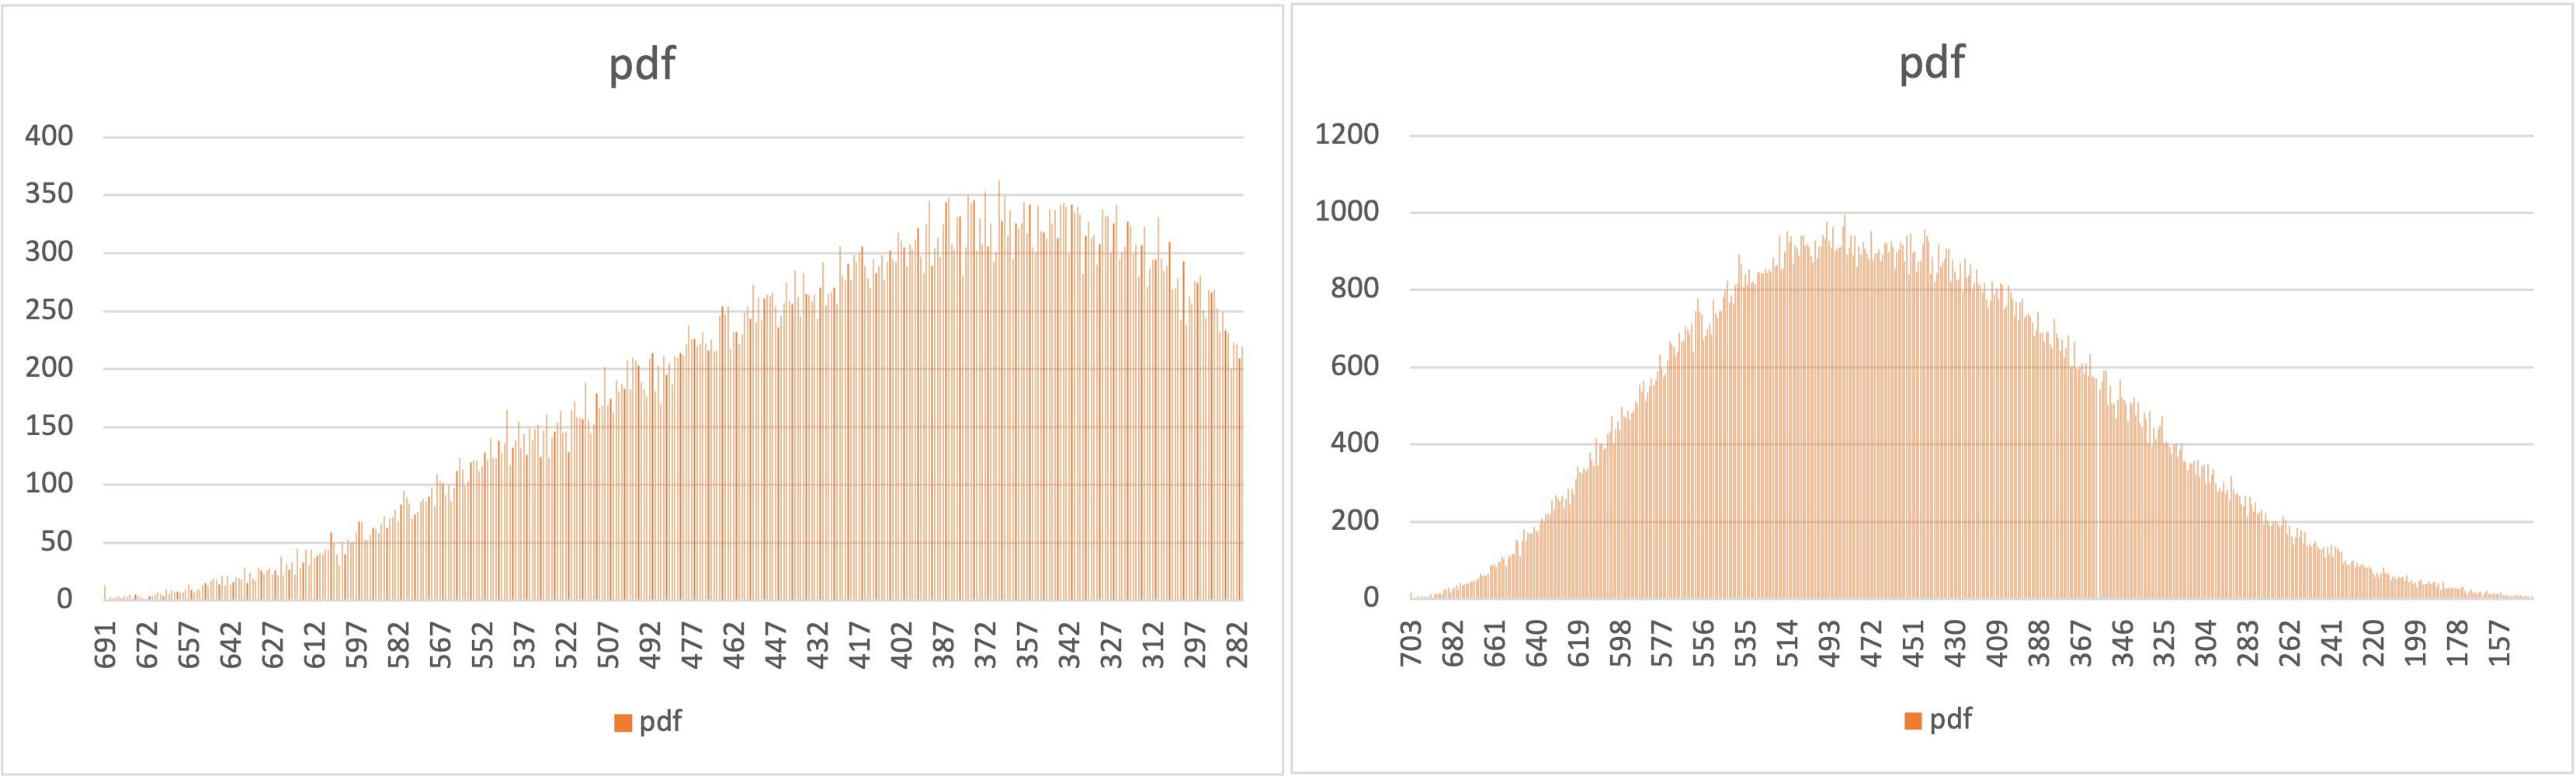
\includegraphics[width=0.9\textwidth]{pdf.png}
\end{figure}

The left figure is Inner Mongolia, the right figure is Hebei province. The average exam score in Hebei is higher than Inner Mongolia, indicating the fiercer competition in Hebei province. Moreover, empirical distribution in Hebei province is approximately normal. But the empirical distribution in Inner Mongolia is skewed.
\section{Admission rate}
In 2023, the cutoff score for tier one universities in Inner Mongolia is 434 (out of 750). There are in total 380 tier one universities accepting applications from Inner Mongolia. The total number of tier one seats is 23587, but there are 28969 students whose exam scores are no less than the tier one cutoff score. So the admission rate of tier one is 81.42\%. The overall admission rate for tier one two and three is about 50\% in Inner Mongolia 2023.

\section{Group size}
\begin{figure}
\centering
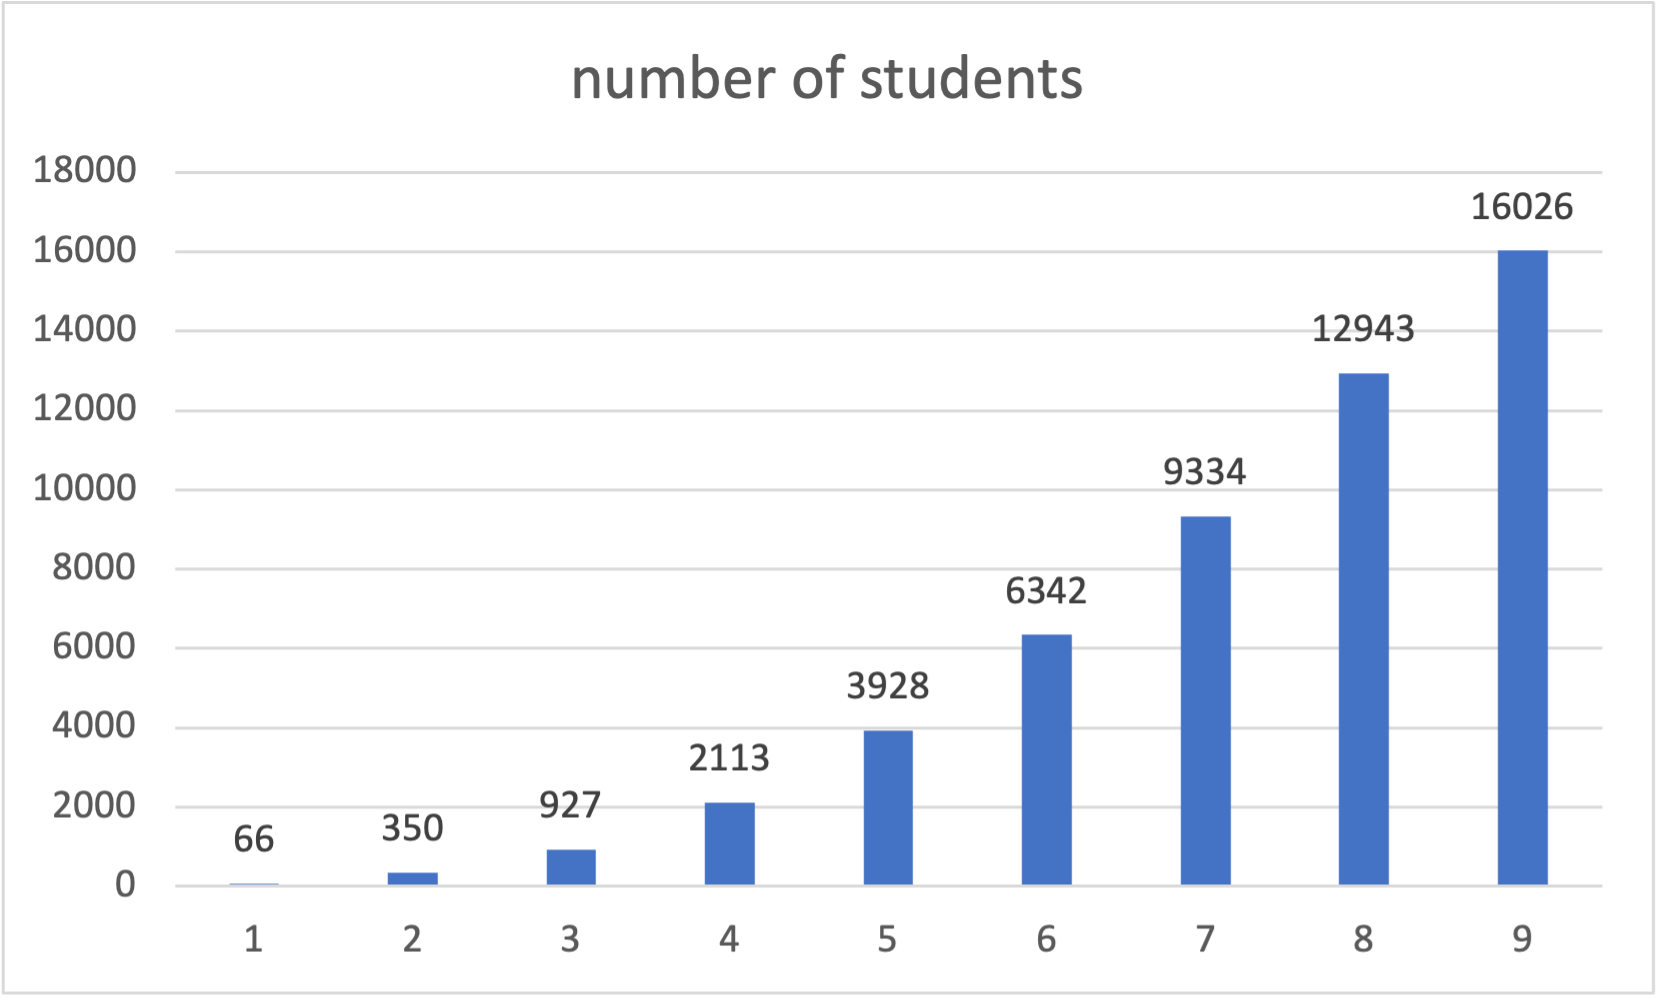
\includegraphics[width=0.9\textwidth]{1.png}
\end{figure}

In the tier one admission market, students are divided into nine groups depending on their exam scores. Every 30 points form a group. Each group move sequentially with one hour constraint. As shown by the above figure, the number of students is increasing across groups aprroximately exponentially.



\end{document}